\section{Position-sensitive detector}

% TODO: lateral photoeffect Schottky30, Wallmark57

\subsection{Transverse photoeffect}

% TODO: cite Simon13

\begin{figure}[H]
	\centering
	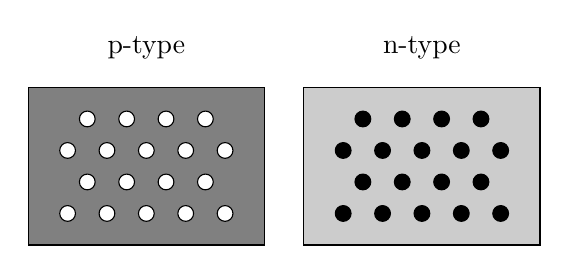
\begin{tikzpicture}
		\draw (1.5, 2.5) node {p-type};
		\draw (5, 2.5) node {n-type};
		\filldraw[draw=black, fill=gray] (0, 0) rectangle (3, 2);
		\filldraw[draw=black, fill=gray!40] (3.5, 0) rectangle (6.5, 2);
		\filldraw[fill=white] (0.5, 0.4) circle (.1) ++(0.5, 0) circle (.1) ++(0.5, 0) circle (.1) ++(0.5, 0) circle (.1) ++(0.5, 0) circle (.1);
		\filldraw[fill=white] (0.75, 0.8) circle (.1) ++(0.5, 0) circle (.1) ++(0.5, 0) circle (.1) ++(0.5, 0) circle (.1);
		\filldraw[fill=white] (0.5, 1.2) circle (.1) ++(0.5, 0) circle (.1) ++(0.5, 0) circle (.1) ++(0.5, 0) circle (.1) ++(0.5, 0) circle (.1);
		\filldraw[fill=white] (0.75, 1.6) circle (.1) ++(0.5, 0) circle (.1) ++(0.5, 0) circle (.1) ++(0.5, 0) circle (.1);
		\filldraw[fill=black] (4.0, 0.4) circle (.1) ++(0.5, 0) circle (.1) ++(0.5, 0) circle (.1) ++(0.5, 0) circle (.1) ++(0.5, 0) circle (.1);
		\filldraw[fill=black] (4.25, 0.8) circle (.1) ++(0.5, 0) circle (.1) ++(0.5, 0) circle (.1) ++(0.5, 0) circle (.1);
		\filldraw[fill=black] (4.0, 1.2) circle (.1) ++(0.5, 0) circle (.1) ++(0.5, 0) circle (.1) ++(0.5, 0) circle (.1) ++(0.5, 0) circle (.1);
		\filldraw[fill=black] (4.25, 1.6) circle (.1) ++(0.5, 0) circle (.1) ++(0.5, 0) circle (.1) ++(0.5, 0) circle (.1);
	\end{tikzpicture}
	\caption{p- and n-type semiconductor separated by a gap}
\end{figure}

\begin{figure}[H]
	\centering
	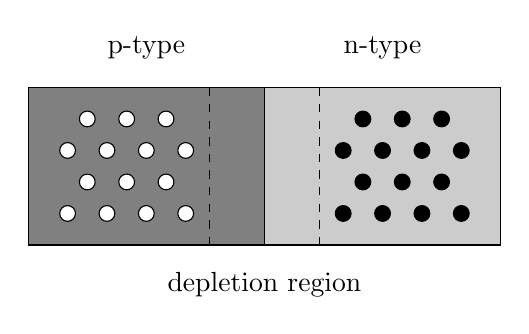
\begin{tikzpicture}
		\draw (1.5, 2.5) node{p-type};
		\draw (4.5, 2.5) node{n-type};
		\filldraw[draw=black, fill=gray] (0, 0) rectangle (3, 2);
		\filldraw[draw=black, fill=gray!40] (3, 0) rectangle (6, 2);
		\filldraw[fill=white] (0.5, 0.4) circle (.1) ++(0.5, 0) circle (.1) ++(0.5, 0) circle (.1) ++(0.5, 0) circle (.1);
		\filldraw[fill=white] (0.75, 0.8) circle (.1) ++(0.5, 0) circle (.1) ++(0.5, 0) circle (.1);
		\filldraw[fill=white] (0.5, 1.2) circle (.1) ++(0.5, 0) circle (.1) ++(0.5, 0) circle (.1) ++(0.5, 0) circle (.1);
		\filldraw[fill=white] (0.75, 1.6) circle (.1) ++(0.5, 0) circle (.1) ++(0.5, 0) circle (.1);
		\filldraw[fill=black] (4.0, 0.4) circle (.1) ++(0.5, 0) circle (.1) ++(0.5, 0) circle (.1) ++(0.5, 0) circle (.1);
		\filldraw[fill=black] (4.25, 0.8) circle (.1) ++(0.5, 0) circle (.1) ++(0.5, 0) circle (.1);
		\filldraw[fill=black] (4.0, 1.2) circle (.1) ++(0.5, 0) circle (.1) ++(0.5, 0) circle (.1) ++(0.5, 0) circle (.1);
		\filldraw[fill=black] (4.25, 1.6) circle (.1) ++(0.5, 0) circle (.1) ++(0.5, 0) circle (.1);
		\draw[dashed] (2.3, 2) -- (2.3, 0);
		\draw[dashed] (3.7, 2) -- (3.7, 0);
		\draw (3, -.5) node[align=center]{depletion region};
	\end{tikzpicture}
	\caption{p- and n-type semiconductor combined to a junction.}
\end{figure}


\begin{equation}
	I_\text{diode}=I_\text{saturation}\left(e^{e_0V_d/k_BT}-1\right)
\end{equation}

% TODO: band diagram
% TODO: band diagram with reverse bias
% TODO: band diagram with illumination

\subsection{Lateral photoeffect}

The lateral photoeffect was first discovered by W. Schottky in 1930~\cite{Schottky30}.
In 1957, it was rediscovered by J. Wallmark~\cite{Wallmark57}.

% TODO: Lucovsky equations Woltring paper
% TODO: pin-cushion type Doke87, Wang89
% TODO: overview of position-sensitive detectors and why we choose the lateral pin-cushion type
% TODO: diagram of depletion region for lateral photodiode


% TODO: photodiode characteristics
% TODO: diode leakage current
% TODO: responsitivity
% TODO: bandwidth limit
% TODO: motivate value for reverse bias

% TODO: noise model
% TODO: photon shot noise

\begin{figure}[H]
	\centering
	\begin{circuitikz}
		\draw (0, 0) node[circ]{};
		\draw (+2, +2) node[ocirc, label=X1]{} to[photodiode] (0, 0);
		\draw (-2, -2) node[ocirc, label=X2]{} to[photodiode] (0, 0);
		\draw (+2, -2) node[ocirc, label=Y2]{} to[photodiode] (0, 0);
		\draw (-2, +2) node[ocirc, label=Y1]{} to[photodiode] (0, 0);
		\draw (0, 0) -- ++(0, -2.5) node[ocirc, label=Cathode, rotate=180]{};
	\end{circuitikz}
	\caption{Position-sensitive detector as photodiodes}
\end{figure}

% TODO: mention non-linearity of voltage response to illumination

\begin{figure}[H]
	% TODO: add position dependent potentiometers to anode (Andersson08 Fig. 15) 
	\centering
	\begin{circuitikz}
		\draw (-3, -2) to[current source, l=$I_\text{photo}$] ++(0, 4);
		\draw (-1, -2) node[circ]{} to[current source, l=$I_\text{dark}$] ++(0, 4) node[circ]{};
		\draw (1, -2) node[circ]{} to[resistor, l=$R_d$] ++(0, 4) node[circ]{};
		\draw (3, -2) to[capacitor, l=$C_d$] ++(0, 4);
		\draw (-3, -2) -- ++(6, 0);
		\draw (-3, 2) -- ++(6, 0);
		\draw (0, -2) -- ++(0, -1) node[ocirc, label=Cathode, rotate=180]{};
		\draw (0, 2) -- ++(0, 1) node[ocirc, label=Anode]{};
	\end{circuitikz}
	\caption{Photodiode equivalent circuit}
\end{figure}